%%%%%%%%%%%%%%%%%%%%%%%%%%%%%%%%%%%%%%%%%%%%%%%%%%%%%%%%%%%%%%%%%%%%%%%%%%
%%%%%%%%%%%%   CAPTER 2   %%%%%%%%%%%%%%%%%%%%%%%%%%%%%%%%%%%%%%%%%%%%%%%%
%%%%%%%%%%%%%%%%%%%%%%%%%%%%%%%%%%%%%%%%%%%%%%%%%%%%%%%%%%%%%%%%%%%%%%%%%%
\chapter{Background and Related Work}
\label{chap:related_work}
%

%%% TODO: eine Seite füllen %%%
While we discussed the developers need for accurate information in the last chapter, we are going to talk about the current state of systems that provide information to developer. There are some well known open source projects, that already collect information and transmit them to evaluation server. We will have a look at how these systems operate and which drawbacks they bring.
To discuss these systems, we start this chapter with an overview of regulations, define which type of data needs special care and how to publish relevant data (section \ref{sec:related:data_aononymization}).\\ 
The next section is related to anonymized and secure data transmission technologies. In section \ref{sec:related:data_transmission} technologies like overlay networks like Tor, which provides user anonymization with the utilization of a wide spread network of nodes, through which participants data is transmitted. To the responding server the request looks like it was send from the exit node and not the original sender. The domain name system is also dissected in this section as it allows a transmission of data to a server without it having knowledge about the origin of the name lookup.
Furthermore we are going to debate how different projects collect user data in section \ref{sec:related:related_sw}. These projects are the Ubuntu Linux distribution, two browser with focus on privacy and a tool designed to collect extensive information on user equipment.
All these different applications use different techniques to strip personal identifiable information, which is added due to transmission from the collected data.

\newpage

%%%%%%%%%%%%%%%%%%%%%%%%%%%%%%%%%%%%%
%%%%%%%%%%%%%%%%%%%%%%%%%%%%%%%%%%%%%
%%%%%%%%%%%%   SECTION   %%%%%%%%%%%%
%%%%%%%%%%%%%%%%%%%%%%%%%%%%%%%%%%%%%
%%%%%%%%%%%%%%%%%%%%%%%%%%%%%%%%%%%%%
\section{Data Anonymization}
    \label{sec:related:data_aononymization}
    %
    
    \subsection{Personal Identifiable Information}
        The US National Institute of Standards and Technology (NIST) defines personal identifiable information as "any information about an individual maintained by an agency, including (1) any information that can be used to distinguish or trace an individual‘s identity, such as name, social security number, date and place of birth, mother‘s maiden name, or biometric records; and (2) any other information that is linked or linkable to an individual, such as medical, educational, financial, and employment information"\cite{mccallister_guide_2010} based on the Government Accountability Office Report GAO-08-536\cite{government_accountability_office_privacy_2008}.\\
        NIST provides a list of information, which can be PII in \cite{mccallister_guide_2010}. This list includes internet protocol (IP) and media access control (MAC) addresses. While the public IP address of an individual device may change over time, the MAC address is a unique device identifier, which is propagated in a network section.
        The IP address may be used to track activities of person over the internet which might have consequences for that persons security and privacy. 
        The MAC address allows the exact identification of a device. It consists of 48 Bytes of which the first 24 Bytes are a vendor identification number. The second 24 Bytes are a unique device identifier from that vendor.\\
        Whilst these two are the most obvious personal dates, other parts of a system may identify 
        a given system uniquely in combination with other data. For example the exact amount of memory in byte or kilobyte may be one of these identifier. How to prevent this kind of linking of published data will be discussed later in this chapter.\\
        
        The Organisation for Economic Co-operation and Development (OECD) provides some guidelines on how to handle personal data in their 2013 privacy framework\cite{oecd_oecd_2013}. These guidelines can be seen in figure \ref{fig:oecd_guide} 
        \begin{figure}
            \centering
            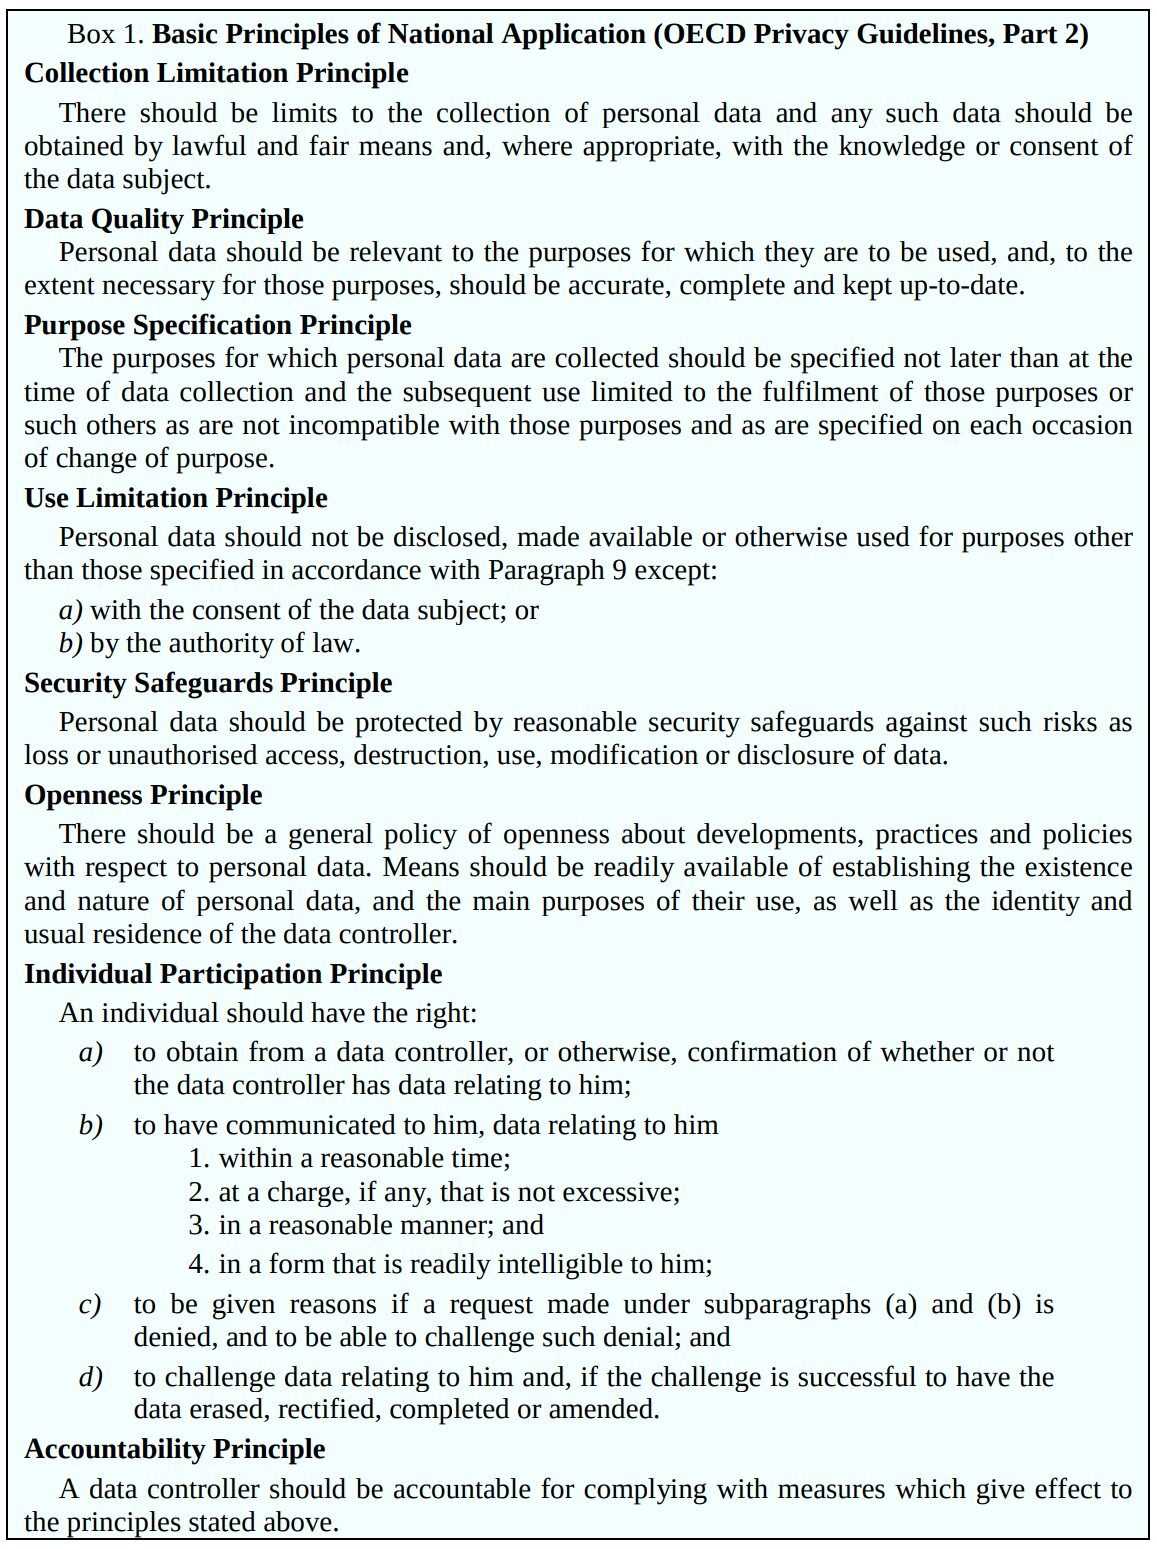
\includegraphics[width=\textwidth]{latex/figures/oecd_guidelines.jpg}
            \caption[OECD guideline]{OECD guideline\cite{oecd_oecd_2013}}
            \label{fig:oecd_guide}
        \end{figure}
        The first principle is the Collection Limitation Principle. It states, that "There should be limits to the collection of personal data [..]"\cite{oecd_oecd_2013}. This principle is reflected in NISTs Guide to protecting the confidentiality of Personally identifiable information\cite{mccallister_guide_2010}. In there it is recommended to minimize the the use, collection and storage of personal data to the minimum necessary to serve its purpose.
        That way, the damage done on a possible data breach is minimized. It is also recommended to review the collected PII previously. If it is no longer relevant, it should be removed\cite{mccallister_guide_2010}.\\
        As a step to protect data sets the NIST guide also recommends de-identification of information. Data with enough PII removed or obscured is treated as de-identified. For this purpose, one-way cryptographic functions (hash functions) may be used\cite{mccallister_guide_2010}.\\
        If there is no code or other association to re-identify, the information as defined as anonymized\cite{mccallister_guide_2010}. This matches with the definition of Anonymity and anonymization.


    \newpage
    %
    %%%%%%%%%%%%%%%%%%%%%%%%%%%%%%%%%%%%%
    %%%%%%%%%%%% Subsection %%%%%%%%%%%%%
    %%%%%%%%%%%%%%%%%%%%%%%%%%%%%%%%%%%%%
    %
    \subsection{Regulations}
        \label{subsec:related:law}
        Anonymity is defined by DIN EN ISO/IEC 29100 as an information characteristic, that does not allow to identify a person directly or indirectly\cite{german_institute_for_standardization_din_2020}. It furthermore declares anonymization as a process, in which personally identifiable information is irrevocable transformed. This transformation denies the ability for an entity to identify a person indirectly or directly by itself or in cooperation with another entity\cite{german_institute_for_standardization_din_2020}.\\
        
        A major advantage for anonymized data is the exclusion of the GDPR legislation. Recital 26 of the regulation excludes anonymized data explicitly.\\ 
        "The principles of data protection should therefore not apply to anonymous information, namely information which does not relate to an identified or identifiable natural person or to personal data rendered anonymous in such a manner that the data subject is not or no longer identifiable. This Regulation does not therefore concern the processing of such anonymous information, including for statistical or research purposes."\cite{european_union_regulation_2016}\\
        Compared to the EU, the US have a wide range of privacy state laws. While the EU aims to provide one general regulation, the US privacy laws are split over four mayor regulations.
        These four are the \textit{Health Insurance Portability and Accountability Act (HIPPAA)}\cite{rights_ocr_summary_2009}, which regulates healthcare provider, \textit{NIST 800-171}\cite{ross_protecting_2015}, that defines how to handle controlled unclassified Information in non-federal information systems, the \textit{The Gramm-Leach-Bliley Act (GLBA)}\cite{noauthor_gramm-leach-bliley_2013}, protecting personal information stored by financial institutes and the \textit{Federal Information Security Management Act (FISMA)}\cite{carper_s2521_2014} in which the requirements are stated for federal agencies information security programs. On top of these, states have additional privacy laws, which may be up to the GDPRs protection, depending on the state\cite{andrada_coos_eu_nodate}.\\
        The European data protection regulation provides a strong set of rules, these may be extended by member state laws, but not weakened. This allows for even stronger data protections in some European countries.
        
    %
    %%%%%%%%%%%%%%%%%%%%%%%%%%%%%%%%%%%%%
    %%%%%%%%%%%% Subsection %%%%%%%%%%%%%
    %%%%%%%%%%%%%%%%%%%%%%%%%%%%%%%%%%%%%
    %
    \subsection{Private Data Publication}
        \label{subsec:related:private_data_analysis}
    
        \subsubsection{\textit{k}-anonymity}
            \label{subsec:related:kanon}
            To avoid the identification of a user, based on the published data and it's attributes, record linkage should not be possible. Therefore a system design should consider so-called quasi identifier (QI). These Quasi identifier may allow to draw a connection between the data set and an external source\cite{sweeney_k-anonymity_2002}.
            If an set of attributes is contained in an external release, that might contain PII, and contained in a released data set, these sets of attributes are called Quasi identifiers, as it allows the linkage between these two data sets.
            If a data set S has $QI_S$ associated with it, S satisfies \textit{k}-anonymity if each sequence of values S[$QI_S$] appears at least \textit{k} times. 
        	In addition, each sequence S[$QI_S$] need to belong to a different user.
        	This does protect the data set against linking, by using direct matching, as Sweeny proposes in \cite{sweeney_k-anonymity_2002}.\\
            
            One of the shortcomings of \textit{k}-anonymity is, that each tuple of attribute need to belong to a different user as Fung demonstrates in \cite{fung_introduction_2011}.

        \subsubsection{\textit{l}-diversity}
            \label{subsec:related:l-div}
            In \cite{machanavajjhala_l-diversity_2007} Machanavajjhala et al. show, that k-anonymity is susceptible the two attack vectors homogeneity and background knowledge.
            The homogeneity attack works on datasets with groups that lack diversity in sensitive attributes. The background knowledge attack on the other hand uses available knowledge in addition to the provided dataset, that is not directly matched to attributes.\\
            

        % differential privacy
        \subsubsection{Differential Privacy}
            \label{subsec:related:dif_privacy}
            Differential privacy (DP) is a property of the data access mechanism and unrelated to auxiliary information available\cite{dwork_algorithmic_2013}. 
            It promises, that the addition, or removal of a single dataset to an existing database does not affect the outcome of a analysis with a strong mathematical definition of privacy. A protection against privacy attacks like re-identification, record linkage and differencing is mathematically provable provided \cite{agrawal_differential_2008}, \cite{wood_differential_2018}. \\
            This guarantees, that anyone will make the same inference about a individuals PII or private information whether the individuals dataset was included in the analysis or not\cite{wood_differential_2018}. Therefore making a post-processing impossible as an analyst can not make the output less differential private without additional knowledge of the the private database\cite{nguyen_understanding_2019}.
            
%%%%%%%%%%%%%%%%%%%%%%%%%%%%%%%%%%%%%
%%%%%%%%%%%%%%%%%%%%%%%%%%%%%%%%%%%%%
%%%%%%%%%%%%   SECTION   %%%%%%%%%%%%
%%%%%%%%%%%%%%%%%%%%%%%%%%%%%%%%%%%%%
%%%%%%%%%%%%%%%%%%%%%%%%%%%%%%%%%%%%%
\section{Data Transmission}
    \label{sec:related:data_transmission}
    %
    The Tor Project is probably the most known approach for anonymized data transmission over the Internet. Besides Tor we are going to discuss different approaches to transmit data over a network. In \ref{subsec:related:overlay} the Tor and I2P overlay network are going to be discussed, followed by domain name system in section \ref{subsec:related:dns}. 
        
        
    %
    %%%%%%%%%%%%%%%%%%%%%%%%%%%%%%%%%%%%%
    %%%%%%%%%%%% Subsection %%%%%%%%%%%%%
    %%%%%%%%%%%%%%%%%%%%%%%%%%%%%%%%%%%%%
    %
    %%%% Overlay Networks
    %
    \subsection{Overlay Networks}
        \label{subsec:related:overlay}
        %
        There are several overlay networks which provide different functionalities, like caching overlays, that enhance the serving static content, routing overlays, that provide different features for dynamic content than the underlying networks and security overlays,  that improve the security of networks and can help mitigate distributed denial of service (DDoS) attacks\cite{pathan_overlay_2014}.\\
        Two overlay networks will be discussed. On the one hand there is Tor\cite{dingledine_tor_2004}, on the other I2P\cite{}. Both systems aim to enhance the anonymity of the internet by adding additional layers to it.\\
        Furthermore additional Protocols like P5\cite{sherwood_p_2005} and Herbivore\cite{goel_herbivore_2003} have been reviewed. As they are similar to the presented solutions, but are less known, or require additional implementation steps or infrastructure, they are not described in this section.
     
     
    %%% Tor %%%
    \subsubsection{Tor}
        The so called Onion Routing used  by Tor is an distributed overlay network to anonymize TCP-based applications. On it's path from sender to receiver, each step in the network only knows it's predecessor and successor. Therefore Information is layered and secured with symmetric keys, which are unwrapped at each step, like the layer of an onion.
        Tor provides perfect forward secrecy by negotiating session keys with each successive hop. If one hop gets compromised, after the keys are deleted, old traffic can't be decrypted\cite{dingledine_tor_2004},\cite{borisov_shining_2008}.\\
        Tor requires some additional work on the client site to configure and setup. 
        The network is operated by a wide variety of people and organizations.
        Thousands of relay nodes are used to route traffic from the origin to it's receiver. It was in 2009 and is of today the biggest network designed for anonymity in operation\cite{edman_anonymity_2009}.
        Therefore it is independent of the collecting entity. Tors systems provides anonymity for the sender against the server and against an attacker in most cases\cite{arma_one_2009}, \cite{poulsen_feds_2013},\cite{samson_tor_2013},\cite{herrmann_website_2009}.\\
        The use of the Tor network is free of charge and open source software, but connecting to it requires additional setup steps from the user.\\
    
    
    
    %%% I2P %%%
    \subsubsection{The Invisible Internet Project - I2P}
        I2P is an overlay network with privacy-by-design in mind, that is intended to connect services within a closed network.
        Exit proxy-server are available, but not recommended by the developer. Within the network, nodes can communicate in any way they want. I2P is free open source software and can be added to a regular web service, to make it available on the closed network. Each network node has unidirectional inbound and outbound tunnel, and every node is visible on the network. However, the traffic of a node can not be seen by other network participants. The network is decentralized and uses distributed hash tables for a network database and contact information security\cite{i2p_intro_2014}.\\
        To contact another client, a message is send out through it's own outbound tunnel, trying to reach the other clients inbound tunnel. Each client can choose the length of tunnels and thereby finding a trade-off between latency and anonymity\cite{anoncoin_i2p_2018}.\\
        I2P requires additional software or setup steps on the client and server side to access the network.\\
        
        
        
    
    %%% VPN %%%
    \subsubsection{Virtual Private Network - VPN}
        A VPN provides an encrypted connection from the users system to an exit point, the VPN server. For further communication the IP address of the VPN server is used. This may change the country of origin and prevent things like geoblocking or other restrictions imposed from the internet service provider\cite{microsoft_virtual_2009}.\\
        A VPN provides privacy against prying eyes in the path from client to VPN server. It also provides anonymity towards the web service requested. Virtual private networks can be self-hosted, used from for-free provider or payed. To use it, additional steps, like configuration, are required on the users end.\\

    
    %%%%%%%%%%%%%%%%%%%%%%%%%%%%%%%%%%%%%
    %%%%%%%%%%%% Subsection %%%%%%%%%%%%%
    %%%%%%%%%%%%%%%%%%%%%%%%%%%%%%%%%%%%%
    %
    %%%% Special systems
    %
    \subsection{Special Systems}
        \label{subsec:related:special}
        There are already systems available, that have been designed for anonymized data collection and transmission. 
        Two such systems, which are currently in use by major open source web browser are dissected below. In \ref{subsec:related:dns} the domain name system is discussed. It is usually not connected to anonymous data transmission, but provides a reliable way to disconnect the senders IP address from the DNS query.
        %
        
    %%% Prochlo %%%
    \subsubsection{Prochlo}
        Prochlo describes a system architecture for large-scale monitoring of software usage activities. The system uses an "Encode, Shuffle, Analyze" approach. Thereby data is encoded and encrypted on one side. It's also the encoders objective to add noise and take care of the randomness of the collected data\cite{bittau_prochlo_2017}.\\
        Afterwards the data is transmitted to a centralized shuffler. They are responsible for the masking of the data origin by removing metadata (IP address, order and time of arrival).
        The data is held for a prolonged time and transmitted only, when a single data item is hidden in a crowd of similar data items. Therefore shufflers need to be trusted entities and separated from the analyzer\cite{bittau_prochlo_2017}. To add further trustworthiness they should be run by third party. The aggregated and reordered data is send out at random intervals to further increase the decoupling of time of arrival and enhance the privacy of clients.\\
        After transmission the data is decrypted, stored and aggregated by the analyzer. 
        Added noise and fragmentation on the encoder site, as well as shuffling may be sufficient to provide differential anonymity in this system.
        
        Prochlo is developed by Google and used by Chromium, as well as, in modified form, by Brave.
        \begin{figure}[hb]
            \centering
            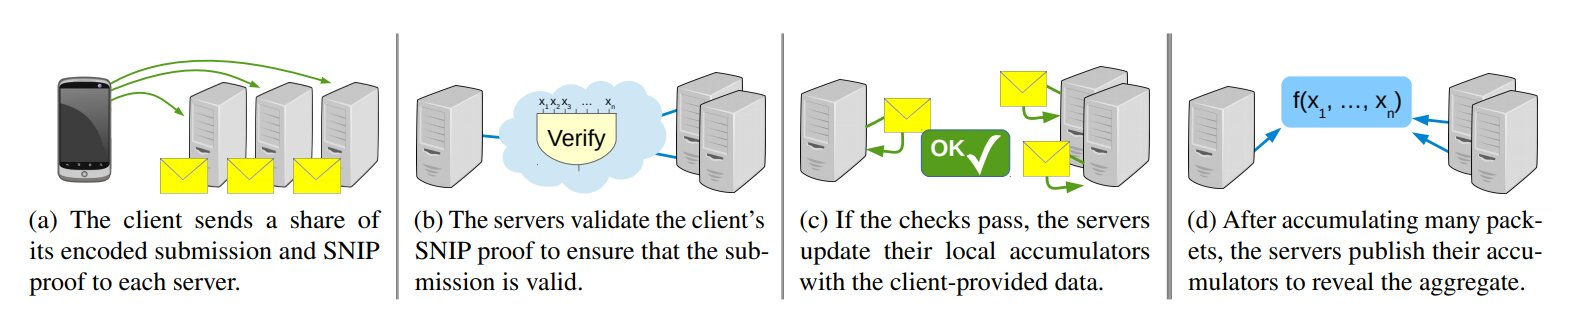
\includegraphics[width=\textwidth]{latex/figures/prio_overview.jpg}
            \caption[Overview of Prios processing pipeline]{Overview of Prios processing pipeline\cite{corrigan-gibbs_prio_2017}}
            \label{fig:prio_overview}
        \end{figure}
    
    %%% Prio
    \subsubsection{Prio}

        Prio was developed by Corrigan-Gibbs et al.\cite{corrigan-gibbs_prio_2017} in 2017 as a privacy-preserving
        system for collecting aggregated statistics
        
        Prio\cite{corrigan-gibbs_prio_2017}, which was developed at Stanford University's Computer Science department for nonsensitive data already covered by their Telemetry tool. 
        Prio splits the collected client data into shares. 
        The parts are send to different servers and aggregated with shares of other users before being published (see figure \ref{fig:prio_overview})\cite{corrigan-gibbs_prio_2017}.\\
        Prio promises privacy, as long as one of the servers is honest, therefore providing strong cryptographic privacy. A limited form of robustness is provided as long as all server are honest. It can detect and discard syntactically incorrect client data while preserving the privacy of the data. However, Prio can not prevent a client from sending in range data, that is untrue\cite{corrigan-gibbs_prio_2017}.\\
        Prio is in experimental use by Firefox Origin Telemetry\cite{englehardt_next_2019}.
        
        
    %%% DNS 
    \subsection{Domain Name System - DNS}
        \label{subsec:related:dns}
        The Domain Name System is hierarchical and decentralized designed to allow systems, connected to a network, to translate memorable domain names into IP addresses\cite{stevens_tcpip_1993}.\\
        \begin{wrapfigure}{Lh}{0.3\textwidth}
            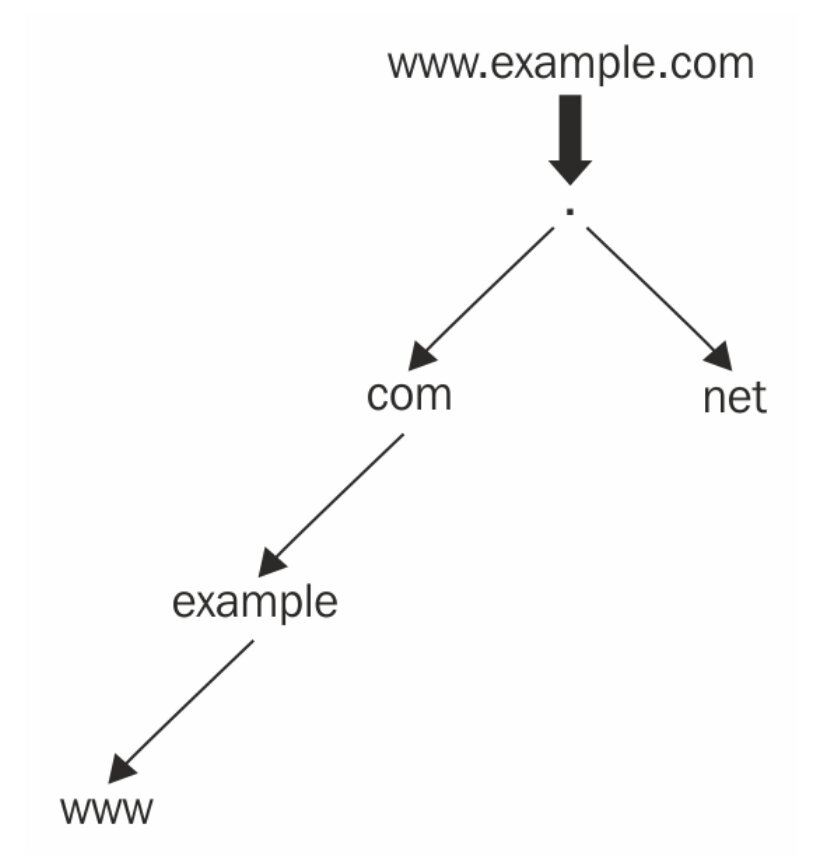
\includegraphics[width=0.3\textwidth]{latex/figures/domain_name_tree.jpg}
            \caption[Domain Name Tree for www.example.com.]{Domain Name Tree for www.example.com. \cite{jeftovic_managing_2018}}
            \label{fig:dns_tree}
        \end{wrapfigure}
        
        This translation is needed, before an application can request a TCP connection or send UDP datagrams. A domain name is a list of labels, separated by dots. 
        Each label can have a length of up to 63 byte, with a maximum length of the requested domain of 255 bytes\cite{stevens_tcpip_1993}.\\
        The dot not only separates each layer in a domain, but is also the internet root, which terminates all Fully QUalified Domain Names (FQDN), but is often omitted\cite{jeftovic_managing_2018}.
        In figure \ref{fig:dns_tree} it is shown, how a hostname can be separated and traversed.
        The first field, following the, here omitted, root entry is the so called Top-Level Domain (TLD). In figure \ref{fig:dns_tree} this would be "com". The root and top-level domain are required to find the responsible authoritative nameserver for any related query\cite{jeftovic_managing_2018}.\\
        

        The name system is structured in non overlapping zones as can be seen in the right segment in figure \ref{fig:dns_query} with the root domain on top\cite{herrmann_beobachtungsmoglichkeiten_2016}.
        A server containing all information about a subset of the name space is called authoritative server. To extract the information from the authoritative server, a so called resolver is used\cite{friedewald_privacy_2018}.
        As the hierarchical structure of the domain name system provides sender anonymity, meaning the receiver doesn't know the source of the message, the system can be used to transmit data anonymously to a collecting server. This can be achieved without any further additions to the protocol or configuration on the client side.
        Advanced techniques like DNS over HTTPS (DoH)\cite{ermert_cloudflare_2020}\cite{mcmanus_dns_2018} or DNS Security Extensions (DNSSEC)\cite{larson_dns_2005} can be used.\\
        DoH uses transport layer security (TLS) to encrypt a connection to a proxy server, which than transmits the DNS request. That way the proxy server the only participant who knows the IP address of the sender. DNSSEC can add another layer of security in protecting against attacks like DNS cache poisoning through adding new components to the DNS system, that check the integrity and authentication of DNS data.\\
        The newly presented Oblivious DNS over HTTPS (ODoH) developed by Apple,Fastly and Cloudflare may add additional privacy to every DNS query and removes one weakness from DoH\cite{verma_improving_2020}.\\
        In ODoH the client encrypts its DNS request for a target server and sends this encrypted message to the proxy server, which than relays the message to the target server. This procedure removes the original request from the clients IP, making the proxy unaware of it.
    At the same time the target server only knows the IP of the proxy as the source. The response is than encrypted for the client and relayed through the proxy.\cite{verma_improving_2020}.
        
        
        
        %%% TODO: citation for DOH and DNSSec
        
        \begin{figure}
            \centering
            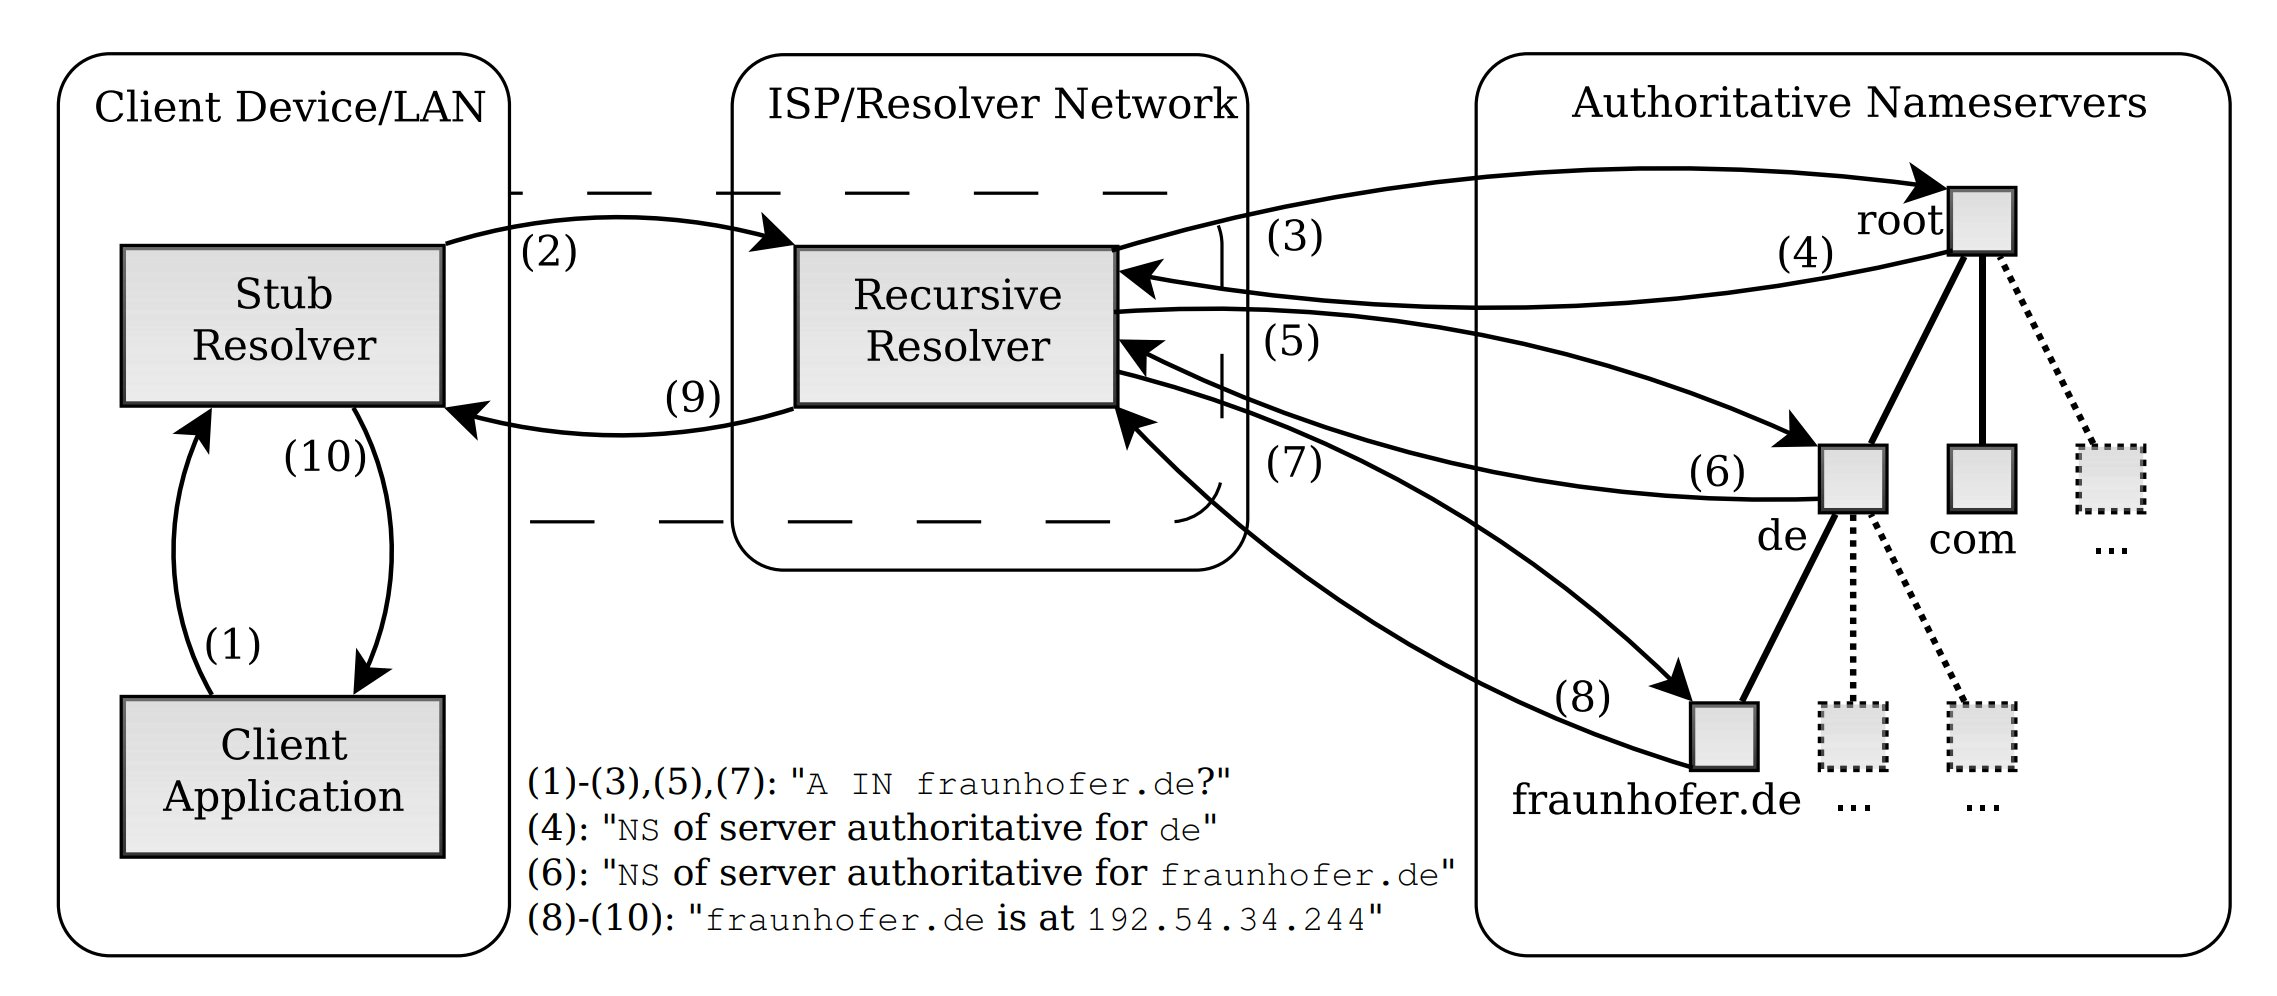
\includegraphics[width=\textwidth]{latex/figures/dns_query.jpg}
            \caption[Full DNS Query with resolver for www.fraunhofer.de]{Full DNS Query with resolver for                 www.fraunhofer.de\cite{friedewald_privacy_2018}}
            \label{fig:dns_query}
        \end{figure}
        
        
        The DNS is also used in Malware for DNS-tunneling or data exfiltration.
        In DNS tunneling \cite{das_detection_2017}.\\
        To exfiltrate data in a DNS request, the information in question is Base32 encoded and split into 63 Byte sized chunks. Afterwards some request are started to a monitored or controlled domain with the encoded data as fields\cite{mertens_infosec_2017}.\\
        
\newpage
%%%%%%%%%%%%%%%%%%%%%%%%%%%%%%%%%%%%%
%%%%%%%%%%%%%%%%%%%%%%%%%%%%%%%%%%%%%
%%%%%%%%%%%%   SECTION   %%%%%%%%%%%%
%%%%%%%%%%%%%%%%%%%%%%%%%%%%%%%%%%%%%
%%%%%%%%%%%%%%%%%%%%%%%%%%%%%%%%%%%%%
\section{Related Software}
    \label{sec:related:related_sw}
    %
    This section introduces some open source projects, that allow data collection, or actively collect user system information. 
    
    %%% Ubuntu %%%
    \subsection{Ubuntu}
        Ubuntu is one of the, if not the, major distributions of the GNU/Linux Operating system. It provides several packages for Server, Desktop or embedded usage. It is used by many major companies on their server\cite{canonical_enterprise_nodate}\\
        Ubuntu collects data with it's "ubuntu-report" tool. By default a system reports its data only once per distribution version. The tools provides a graphical user interface and command line version and prompts the information to the user before sending\cite{roche_ubuntuubuntu-report_2020}.\\
        A JSON report as shown in listing \ref{lst:ubuntu-report} in the Appendix is send to the Ubuntu server, if the user opts in. If the user opts out, a report is created as in listing \ref{lst:opt-out} and send to the Ubuntu server\cite{roche_ubuntuubuntu-report_2020}.\\ 
        \begin{lstlisting}[language=json, caption=JSON report on opt out, label=lst:opt-out]
            {
                "OptOut": true
            }
        \end{lstlisting}
        This allows Canonical to get a relatively precise number of internet connected devices, that run Ubuntu.\\
        There is no PII collected, only data like system architecture, RAM, disk space, monitor count and resolution are reported.\\
        To transmit the data, a HTTP POST is send over TLS to the Ubuntu server.\\
        
        In a HTTP POST the body of the message contains the payload, compared to a GET, where the payload is appended to the URL.
        It is not encrypted or encoded by default, by can be upfront to protect the bodies data from inspection. In addition or instead protocols like TLS can be used to encrypt the transport. But if an attacker knows the session key, all ongoing communication can be read. Prior communication is secured as TLS provides forward secrecy.\\
        
        As this is a TCP direct connection, the public IP address of the sending system can be connected to the collected data on the server side.
        The user must trust the collecting services, that the information is not stored, but discarded.\\
        
    %%% hw-probe %%%
    \subsection{Hardware Probe Tool - hw-probe}
        The Hardware Probe Tool is an open source tool to collect hardware, system and log information on Linux and BSD based systems. It is written in Perl and collected data is available for everyone to see. 9780 unique systems have reported there system information in 2019\cite{ponomarenko_linux_nodate}.
        While serial numbers and MAC addresses are collected, they are salted and hashed with SHA512 and only 32 Byte are transmitted. 
        This should avoid recreation of any personal identifiable information and uniquely identify a system against the database \cite{project_linuxhwhw-probe_2020}.\\
        The collected data can be pretty extensive if a complete collection is enabled. It includes among other things installed drivers, connected PCI devices, system architecture, operating system, network interface type and UUID\cite{project_linuxhwhw-probe_2020}.\\
        
        To transmit the collected data, HTTP POST messages are send to the collection server. The transmissions uses TLS to secure the content of these messages\cite{project_linuxhwhw-probe_2020}.\\
        Again the IP of the system is connected to the data set transmitted and the user has to rely and trust on the collecting entity to separate these two information from each other.\\
    


\newpage
    %%% Firefox %%%
    \subsection{Firefox}
        Firefox is a Browser which promises speed and privacy. It provides advertisement and tracker blocking. In addition it is available on all major platforms\\ 
        By default Firefox collects a wide range of data. These data collections are called Pings. Each Ping contains a certain type of information. At the time of writing there are at least 27 different Ping types in use\cite{mozilla_telemetry_nodate}.
        
        \begin{wrapfigure}{R}{0.4\textwidth}
            \centering
            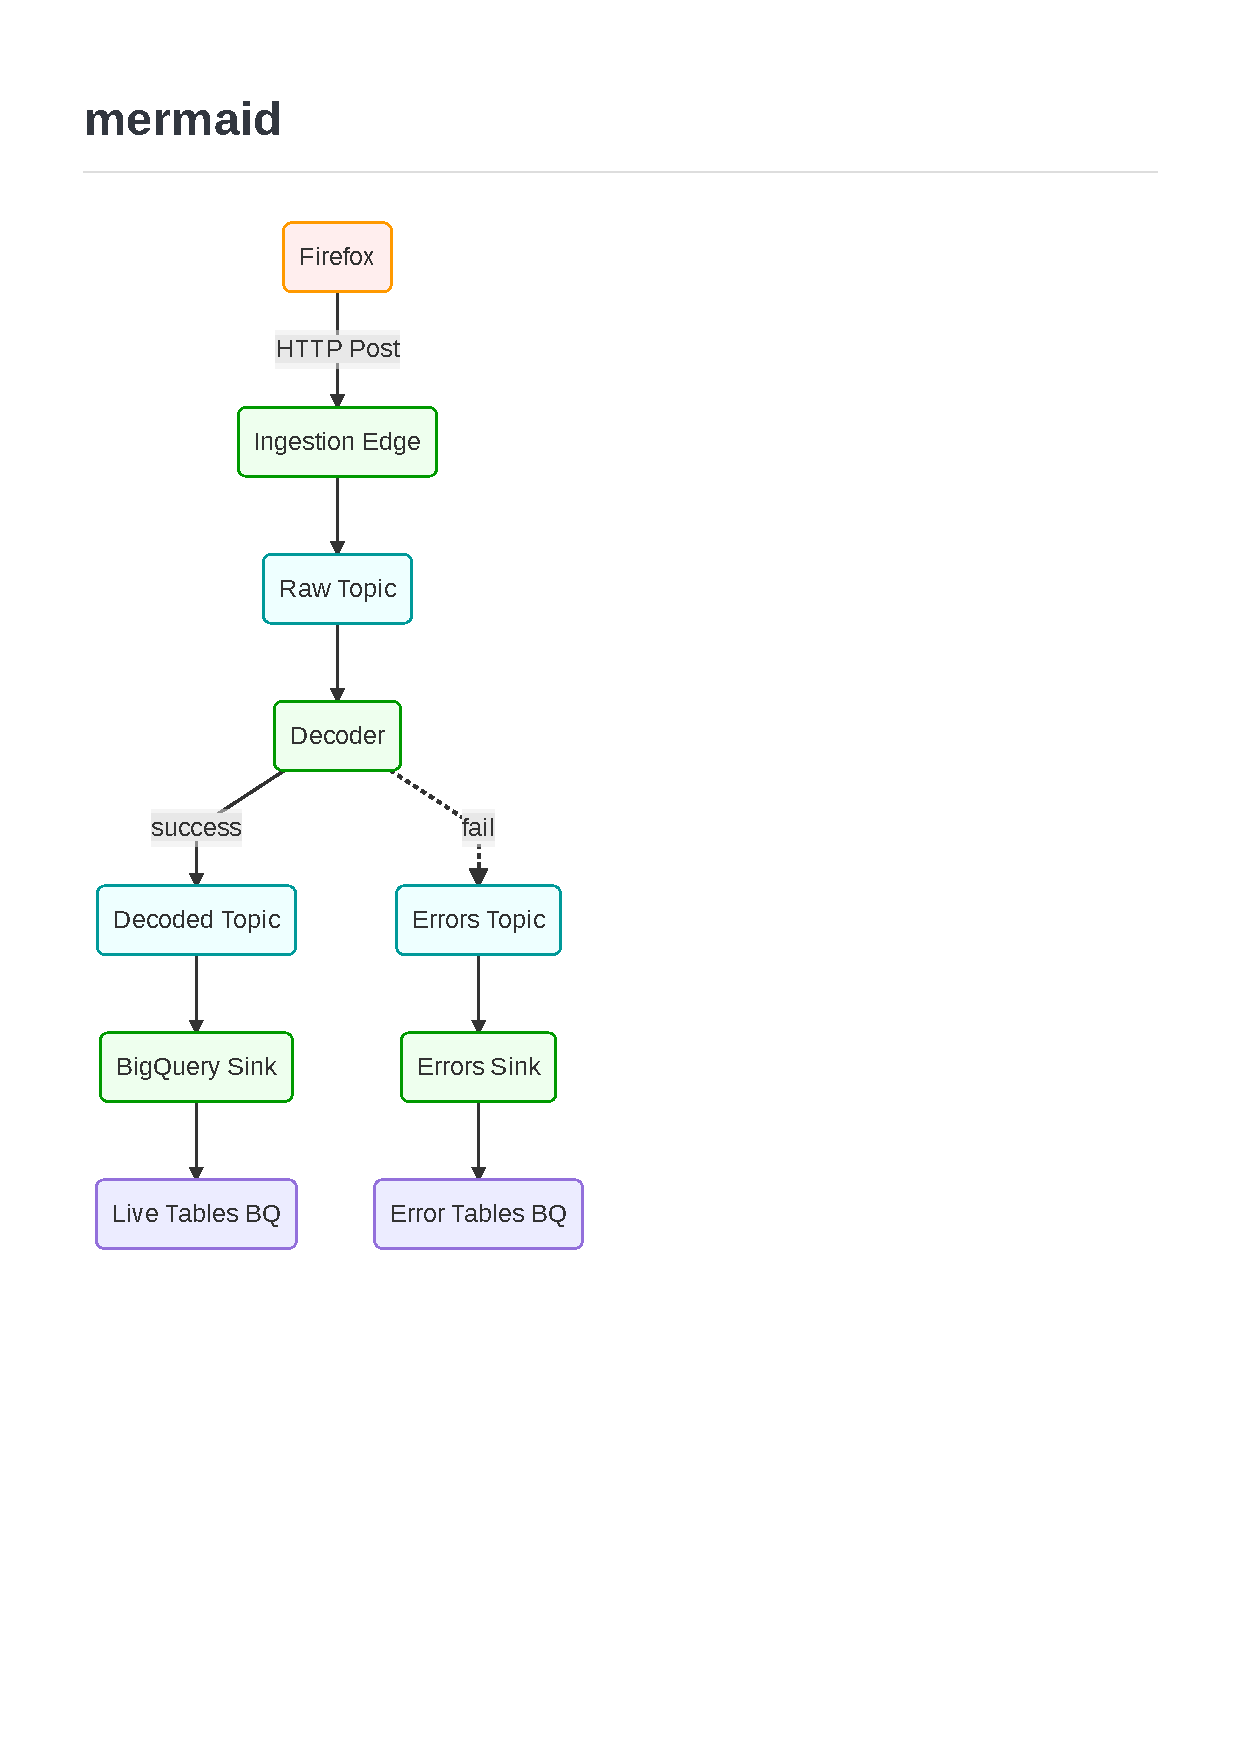
\includegraphics[clip, trim=0.5cm 8cm 8cm 3.5cm, width=0.4\textwidth]{latex/figures/firefox_telemetry_graph}
            \caption[Firefox data flow]{Firefox data flow based on \cite{mozilla_overview_2020}}
            \label{fig:moz_data_flow}
        \end{wrapfigure}
        
        The "main" Ping is used for most telemetric data. It contains extensive health and performance information on Firefox, but also most system information. The JSON structure of a "main" Ping can be seen in Mozillas pipeline schema GitHub repository\cite{mozilla_mozilla-servicesmozilla-pipeline-schemas_2020}. 
        Besides information on CPU, GPU and operating system it contains information on installed add-ons and the reason for sending the Ping.
        It is send at least every 24 hours, but also on startup and other occasions. While basic telemetry, like the main ping can be disabled on the Settings page, Firefox will still send selected Pings to it's server, unless disabled in \textit{about:config}.
        %TODO: verify with wireshark - firefox sends stupid amount of data
        To send the collected Telemetry, Firefox uses a program called Ping Sender.
        This will send a HTTP POST to the Edge Server where it is forwarded to the data pipeline if it's is formatted correctly.
        If a client IP address is available at the decoder, the geolocation will be determined and saved.
        The IP address gets discarded from the data set in the process\cite{mozilla_overview_2020},\cite{mozilla_http_2020},\cite{firefox_ping_nodate}.\\
        A reduced data pipeline can be seen in figure \ref{fig:moz_data_flow}.
        
        
        
    
        Mozilla was experimenting with Prio in 2018 \cite{helmer_testing_2018} and based on the experiment they developed Firefox Origin Telemetry \cite{englehardt_next_2019} which is, at the time of writing, in use only for content blocking and still     experimental\cite{noauthor_origin_nodate}.\\
    
    
    %%% Brave %%%
    \subsection{Brave}
        Brave is a free open source browser with a focus on privacy. It provides advertisement and tracker blocking, as well as a Tor integration. It is based on Chromium and promises to be faster than it and claims to have better default privacy than Firefox. It is a relatively new Browser, but already supports all major platforms\cite{brave_secure_nodate}.\\
        Brave uses a technique called Privacy Preserving Product Analytics (P3A) for telemetry data, which can be turned off at any time.
        They claim, that their P3A does cover way more, than expected by GDPR. No personally identifiable data (PII) is collected or transmitted.\\
        Therefore Braves telemetry process is split into two phases.\\
        The first phase consists of several multiple choice questions, for which the answer is send individually.
        Each question poses a number of answers. Quantifiable questions, like the the number of open tabs, provide ranges for each answer for enhanced privacy\cite{brave_privacy-preserving_2019}. These Questions and possible answers can be reviewed in Braves GitHub repository\cite{brave_software_inc_brave-browser_2019}.
        The questions of phase one can be seen in Listing \ref{list:brave_question} in the appendix as well.\\
        At a randomized time after opening the browser, the number of open tabs is counted and send out once an hour with further information\cite{brave_privacy-preserving_2019}.
        An answer contains:
        \begin{itemize}
            \item Question number, Answer number
            \item OS/Platform
            \item Release information (nightly/dev/bet/release)
            \item Week of installation (if installation was within 90 days)
            \item Country (if fewer than 6000 installs per week this is removed)
            \item Referral code (only if within 90 days of install and referrer is big enough)
        \end{itemize}
        Every answer is send to Braves content delivery network (CDN) and stripped of the IP address of the client at the edge of the CDN\cite{brave_privacy-preserving_2019}.
        . 
        The Second Phase uses a protocol based on Prochlo(see \ref{sec:related:data_transmission}. 
        
        The study Leith conducted in February 2020 \cite{leith_web_2020} supports Brave Software Inc. claims
        for a privacy caring browser.\\
        In his survey Leigh evaluated the privacy settings of six browsers (Brave, Chrome, Edge, Firefox, Safari and Yandex) has been compared. While Brave and Firefox (with changed defaults) where strongly focused on privacy all Browser did send there reports in combination with the users IP address\cite{leith_web_2020}.
        This is problematic, as an IP address can be used to pin down the users geolocation\cite{koch_geolocation_2013}. Workplaces or homes can be derived based on the time people spend in places during day or night. 
        While Brave Software Inc. claims, that they remove the IP address at the edge of their CDN, the user has to trust the CDN operator to strip the send data of the address for phase one answers. In Phase two the user has to trust the shuffler to remove the meta data from the collected data. 
\newpage
%%%%%%%%%%%%%%%%%%%%%%%%%%%%%%%%%%%%%
%%%%%%%%%%%%%%%%%%%%%%%%%%%%%%%%%%%%%
%%%%%%%%%%%%   SECTION   %%%%%%%%%%%%
%%%%%%%%%%%%%%%%%%%%%%%%%%%%%%%%%%%%%
%%%%%%%%%%%%%%%%%%%%%%%%%%%%%%%%%%%%%
\section{Summary}
    In this chapter we discussed what personal information are and how they should be handled.
    In addition we summarized previous work on related topics. This allows us to narrow our research.
    Prio and Prochlo require additional infrastructure. As open source organization are usually underfunded, every additional server leaves a dent in the budget. Therefore these systems maybe
    useful for organizations with sufficient funding, but not for small projects. Some of the mentioned systems in this chapter depend on trust of the user that their transmission information are stripped from the data.\\
    
    On the other hand, client side enabled anonymization, like using the tor network or VPNs, may require additional maintenance or knowledge from the user. This could reduce the amount of participating user significantly.\\
    
    The Domain Name System provides us a hierarchical structure, that strips the senders information from the transmitted data in a reliable way. A user, can have trust in that and doesn't depend on an organization to handled that properly while the anonymization process doesn't require any additional knowledge the user must have.\\
    Utilizing DNS for data transmission opens up a range of new issues that need to be handled and will be discussed in the next chapter.\\ 
    
    
%


  